% ****** Start of file apssamp.tex ******
%
%   This file is part of the APS files in the REVTeX 4.1 distribution.
%   Version 4.1r of REVTeX, August 2010
%
%   Copyright (c) 2009, 2010 The American Physical Society.
%
%   See the REVTeX 4 README file for restrictions and more information.
%
% TeX'ing this file requires that you have AMS-LaTeX 2.0 installed
% as well as the rest of the prerequisites for REVTeX 4.1
%
% See the REVTeX 4 README file
% It also requires running BibTeX. The commands are as follows:
%
%  1)  latex apssamp.tex
%  2)  bibtex apssamp
%  3)  latex apssamp.tex
%  4)  latex apssamp.tex
%
\documentclass[%
 reprint,
%superscriptaddress,
%groupedaddress,
%unsortedaddress,
%runinaddress,
%frontmatterverbose,
%preprint,
%showpacs,preprintnumbers,
%nofootinbib,
%nobibnotes,
%bibnotes,
 amsmath,amssymb,
 aps,
%pra,
%prb,
%rmp,
%prstab,
%prstper,
%floatfix,
]{revtex4-1}

\usepackage[utf8]{inputenc}
\usepackage[norsk]{babel}
\usepackage{graphicx}% Include figure files
\usepackage{dcolumn}% Align table columns on decimal point
\usepackage{bm}% bold math
\usepackage[mathlines]{lineno}% Enable numbering of text and display math
%\linenumbers\relax % Commence numbering lines

\usepackage[usenames,dvipsnames,svgnames,table]{xcolor}
\usepackage[colorlinks]{hyperref}
\usepackage{relsize}
\usepackage{amsmath,graphicx,varioref,verbatim,amsfonts,geometry}
\newcommand*\diff{\mathop{}\!\mathrm{d}}
\newcommand*\Diff[1]{\mathop{}\!\mathrm{d^#1}}
\usepackage{ulem}
\usepackage{amssymb}
\usepackage{soul}
\usepackage{dsfont}
\usepackage{commath}
\usepackage{wrapfig}
\usepackage[free-standing-units=true]{siunitx}
\DeclareSIUnit\year{yr}
\usepackage{gensymb}
\newcommand{\ROM}[1]{%
  \textup{\uppercase\expandafter{\romannumeral#1}}%
}
\usepackage{physics}
\usepackage{caption}
\usepackage{bm}

%\usepackage[showframe,%Uncomment any one of the following lines to test
%%scale=0.7, marginratio={1:1, 2:3}, ignoreall,% default settings
%%text={7in,10in},centering,
%%margin=1.5in,
%%total={6.5in,8.75in}, top=1.2in, left=0.9in, includefoot,
%%height=10in,a5paper,hmargin={3cm,0.8in},
%]{geometry}

\begin{document}

%\preprint{APS/123-QED}

\title{Strøm og Spenning}

\author{\textsc{Haugerud, Ivar Svalheim}}
\affiliation{%
 University of Oslo\\
}%

\date{\today}

\begin{abstract}
We need to test if our system behaves as it should based on the equations we have in the theory section, which is derived in the appendix. To start with this we visualized the particles in the compartment. Since the visualizing demands more computer power than our computers can handle here at the university of Soby, we had to limit ourselves to only $100$ particles. We saw that the particles behaved as they should, and did bounce on the walls when they were meant to, and it looked like their kinetic energy was conserved.
\end{abstract}

\pacs{Valid PACS appear here}% PACS, the Physics and Astronomy
                             % Classification Scheme.
%\keywords{Suggested keywords}%Use showkeys class option if keyword
                              %display desired
\maketitle

%\tableofcontents
\section{\label{introduksjon}Introduksjon}
Eksperimentet diskutert i denne rapporten ble gjennomført i håp om å finne ut av, og forstå, samspillet mellom komponenter, og effekten komponentene og måleapparatene har på kretsen de er en del av. De følgende kretsene vi skal se på ble lagd for å teste denne effekten. Spenningen i kretsen vil være generte av DA-omformere og oscilloscop, dette lar oss variere frekvens og amplitude som vi ønsker. Dette vil bli målt av multimetere, AD-omformere og oscilloscop. Kretsen kommer i all hovedsak til å bestå av resistanser, kondensatorer og termistorer. Med disse komponentene og måleapparatene kan vi måle hvordan kompoentene oppfører seg i samspill for forskjellige amplituder og frekvenser. Spesielt vil vi se på hvordan kondensatorer oppfører seg for høye og lave frekvenser, og vi kan sammlikne målingene med hva teorien fra Ohm's lov, sammen med kirchhoffs lover, forutsier at resultatene skal være.
\section{\label{teori}Teori}
Vi jobber med elektriske kretser hvor vi bruker Ohm's lov \cite{skaar} for å regne på kretsene våre
\begin{equation}
  V = IR \label{ohm},
\end{equation}
hvor $V$ er spenningsfallet over en komponent, $I$ er strømmen som gjør gjennom komponenten, og $R$ er resistansen til komponenten. Dette gir oss forholdet mellom motstand, strøm og spenningsfall, som er nødvendig for en hver krets. Denne formelen kommer vi til å bruke mye gjennom forsøket siden vi kan finne resistansen ved å måle spenningsfallet over en komponent når vi vet hva strømmen er. Dette blir spesielt nyttig hvis resistansen til en komponent er avhengig av temperaturen i rommet. \\
I kretsene våre kommer vi til å bruke kondensatorer. Kondensatorer kan lagre elektriske ladninger med netto ladning $Q$, dette generer et spenningsforskjell mellom kondensatorplatene $V$. Disse to egenskapene til kondensatoren gir oss kapasitansen til kondensatoren som er gitt av
\begin{equation}
  C = \frac{Q}{V},
\end{equation}
hvor $C$ er kapsitansen. Kapasitansen er bare avhengig av materialet og de geometriske strørrelsene til kondensatorplatene \cite{skaar}. Kapasitansen sier oss hvor mye ladning kondensatoren klarer å oppbevare før den blir \textit{full}. Hvis man kobbler inn en resistanse i kretsen også, slik at man får en RC-krets, vil man ha lagd et lavpassfilter. Grunnen til dette er at forflyttingen av ladninger i kretsen tar tid, og gjør at, hvis man har en vekselstrøm (AC) vil spenningen over kondensatoren være en funksjon av tid, og med for stor frekvens på strømmen vil ikke strømmen i kretsen ha tid til å fylle opp kondensatoren med ladninger før strømmen endres igjen. Og derfor vil man ha en høy frekvens som går inn i kondensatoren, men en lav frekvens som går ut av kondensatoren. Forholdet mellom spenningen inn $V_i$ og spenningen ut $V_u$ kan vises at \cite{oppgave} er
\begin{equation}
  \abs{\frac{V_u}{V_i}} = \frac{1}{\sqrt{1+\left(\frac{\omega}{\omega_0}\right)^2}}
\end{equation}som, ved å ta logarytmen på begge sider, kan skrives om til
\begin{equation}
  \log\abs{\frac{V_u}{V_i}} = -\frac{1}{2}\log\left\{1+\left(\frac{\omega}{\omega_0}\right)^2 \right\}
\end{equation}
Her har spenningen inn en frekvens $\omega$ og $\omega = 1/RC$, som er den karakteristiske frekvens til kretsen. For lave frekvenser ser vi at $\log\abs{V_u/V_i}\approx 0$. For høye frekvenser ser vi at $\log\abs{V_u/V_i}\approx -\log(\omega) + log(\omega_0)$, som, hvis plottet med logaritmiske akser, er en rett linje med konstantledd $\log(\omega_0)$ og stigningstall $-1$, der $x$-aksen er $\omega$ og $y$-aksen er $\abs{V_u/V_i}$. Dette betyr at den relative amplituden faller en faktor $10$ for hver faktor $10$ vi øker frekvensen. Dette gjør at de høye frekvensene vil falle bort, som gjøre kretsen til et lavpassfilter.
\\
Når vi jobber med vekselstrøm (AC) er man ofte interesert i effektverdien, eller RMS-verdien til signalet. Denne verdien er definert som
\begin{equation}
  V_{rms} = \sqrt{\frac{1}{T} \int_0^T V(t)^2 \diff t} \label{rms},
\end{equation}hvor $T$ er tiden for en full periode og $V(t)$ er spenningen i kretsen. Hvis man løser dette integralet for forskjellige signalformer får man RMS-verdien. De signalen vi skal se på er sinussignal, firkantsignal og sagtann signal, det kan vises at RMS-verdiene til signalene er henholdsvis lik $A/\sqrt{2}$, $A$, $A/\sqrt{3}$, hvor $A$ er amplituden av signalet \cite{rms_wiki}.
\\
Et av eksperimentene går ut på å måle resistansen til en temperatursensitiv termistor, der motstanden er en funksjon av temperatur, og ut ifra målingene av resistansen måle temperaturen. Utrykket for dette forholdet er
\begin{equation}
  T(R) = \frac{1}{a+b\, \log R + c \left(\log R\right)^3} - 273.16 \text{C} \label{calc_temp}
\end{equation}hvor $a$, $b$ og $c$ er konstanter. Her sender vi med en resistanse, og får ut en temperatur målt i celcius.
\section{\label{metode1}Metode}
Vi ønsket å finne ut hvordan det å måle motstand, strøm eller spenning påvirker kretsen som måleapparatet er med i. For å gjøre dette brukte vi to multimetere Fluke $75$ (F$75$) som er et håndholdt multimeter, og Fluke $45$ (F$45$), som er et stasjonert multimeter. Vi lot multimeterene måle på hverandre i en ekstremt simpel krets der måleapparatene er de eneste komponentene i kretsen, dette er vist i figur \vref{fig1}. Dette gjorde vi for alle kombinasjonene av resistans, strøm og spenning i kretsen, og varierte sensitiviteten og samplings-frekvensen (slow (S), medium (M) og fast (F)) til måleapparatene. \\
\begin{figure}[h!]
    \centering
    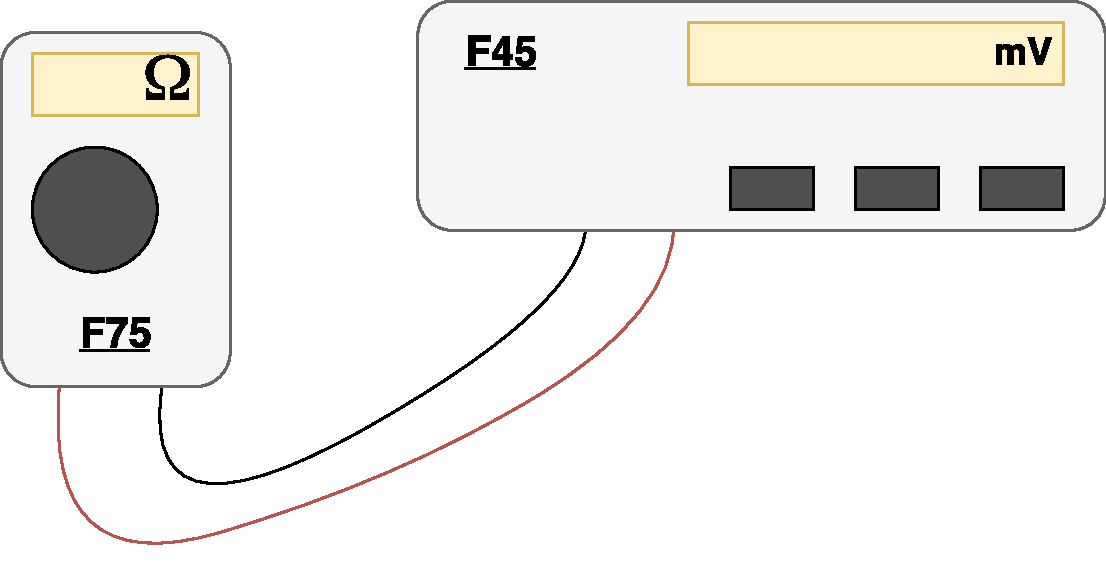
\includegraphics[scale=0.35]{fig_1.pdf}
    \caption{Figur som viser F$45$ og F$75$ som måler på hverandre i en veldig simpel krets. I dette eksempelet måler F$75$ resistansen gjennom kretsen, mens F$45$ måler spenningen.}
    \label{fig1}
\end{figure}
Nå som vi viste hvordan måleapparatene påvirket krets de selv er med i brukte vi dem til å måle resistansen til to motstander hvor vi vist den eksakte verdien av resitansen. Dette gjorde vi ved å sette opp en enkel krets vist i figur \vref{fig2} ved hjelp av et breadbord.
\begin{figure}[h!]
    \centering
    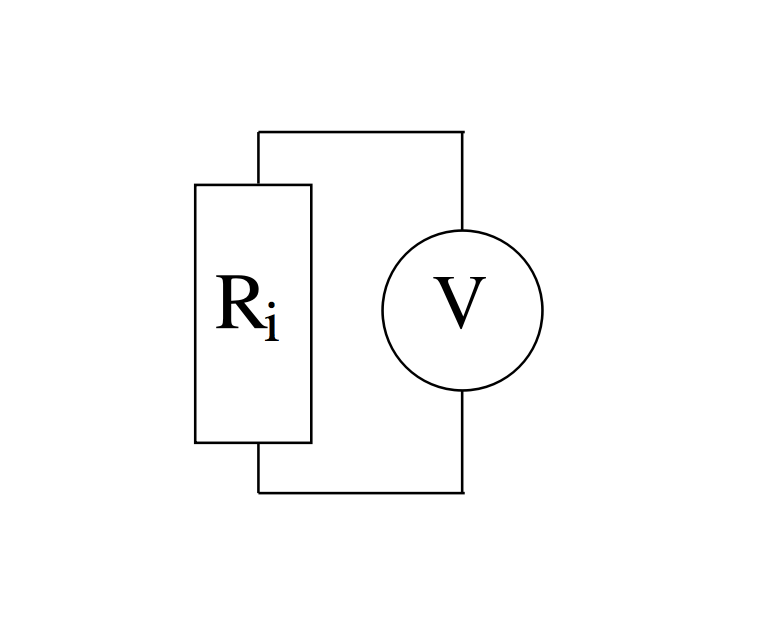
\includegraphics[scale=0.15]{fig_2.png}
    \caption{Krets brukt for å måle resistansen til motstander der vi kunne variere $R_i$.}
    \label{fig2}
\end{figure}
Vi valgte denne kretsen siden dette var den letteste mulige kretsen for hensikten vår. Vi brukte to forskjellige resistanser i kretsen, først $R_1 \sim 10 \Omega$ og så $R_2 \sim 1 M\Omega$. Vi gjorde først målingene med F$75$ og så med F$45$. Hvor begge appartene brukt ohm-funksjonen, slik at de genererte strømmen i kretsen selv.\\
Vi ønsket så å utvide kretsen og gjøre den litt mer komplisert. Kretsen vi lagde er vist i figur \vref{fig3}.
\begin{figure}[h!]
    \centering
    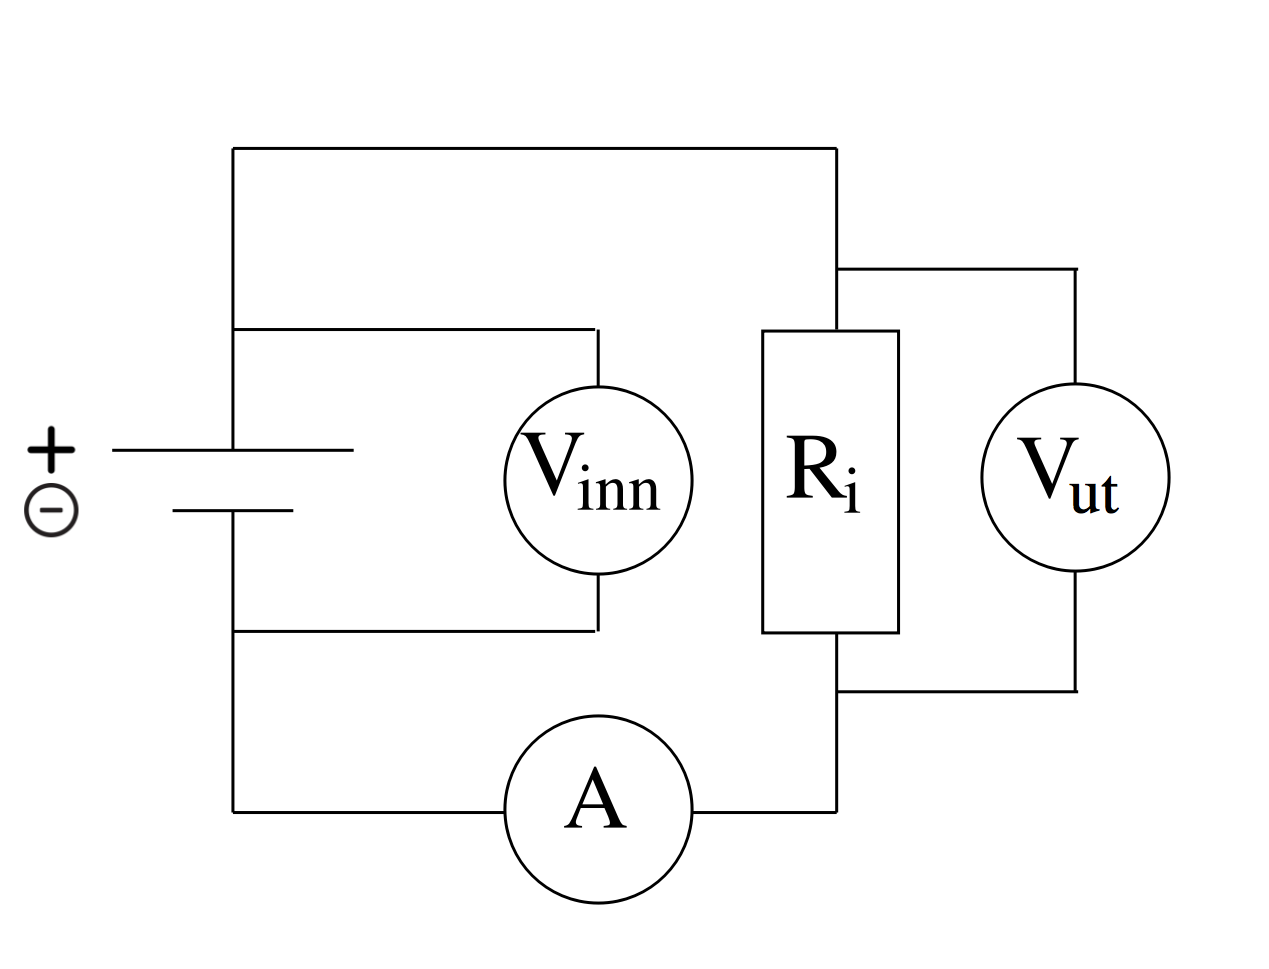
\includegraphics[scale=0.15]{fig_3.png}
    \caption{Krets brukt for å måle resistansen til motstander der vi kunne variere $R_i$.}
    \label{fig3}
\end{figure}
I denne kretsen måler vi spenningsfallet over hele kretsen ved $V_{inn}$, spenningsfallet over resistansen ved $V_{ut}$, og strømmen som går gjennom kretsen ved amperemeteret. Med disse målingene kan vi regne ut resistansen til motstanden. Siden vi hadde to mutlimetere, og tre verdier vi ønsket å måle i kretsen måtte vi koble om kretsen under forsøket for å gjøre de forskjellige målingene. Når alt var riktig koblet opp varierte vi strømmen i kretsen, og gjorde målinger for begge resistanser for hver frekvens. Da vi gjorde målinger med $R=\SI{10}{\ohm}$ brukte vi F$45$ som voltmeter, og F$75$ som amperemeter. Når vi gjorde de samme målingene for $R=\SI{1}{\Mega \Ohm}$ måtte F$45$ være amperemeter, siden F$45$ hadde høyere sensitivitet, og kunne derfor gi målinger på den lave strømmen i kretsen. I kretsen vår brukte vi F$45$ for å måle $V_{inn}$ og $V_{ut}$, mens vi brukte F$75$ som amperemeter, grunnen til dette var at det ga oss minst omkoblinger underveis. \\ \\
Vi ønsket nå å gjøre målinger ved hjelp av en datamaskin for å autmatisere målingene, og få en grafisk fremstilling av dataen. For å få dataen fra målingene inn på datamaskinen koblet vi tre fofrskjellige punkter i kretsen inn til en dataakvisisjonsboks (DAQ, NI USB-6211). I kretsen hadde vi en konstant spenning på $\SI{5}{\volt}$, og en termistor ($R_T$) og en resistans ($R_2$) koblet i serie. Mellom hver av resistansen koblet vi kretsen inn til akvisisjonsboks, kretsen er vist i figur \vref{fig4}. Her er $AIGND$, $AI0$, $AI1$ inngangene vi brukte på akvisasjonsboksen og referanse motstanden $R_2$ var på $1M\Omega$.
\begin{figure}[h!]
    \centering
    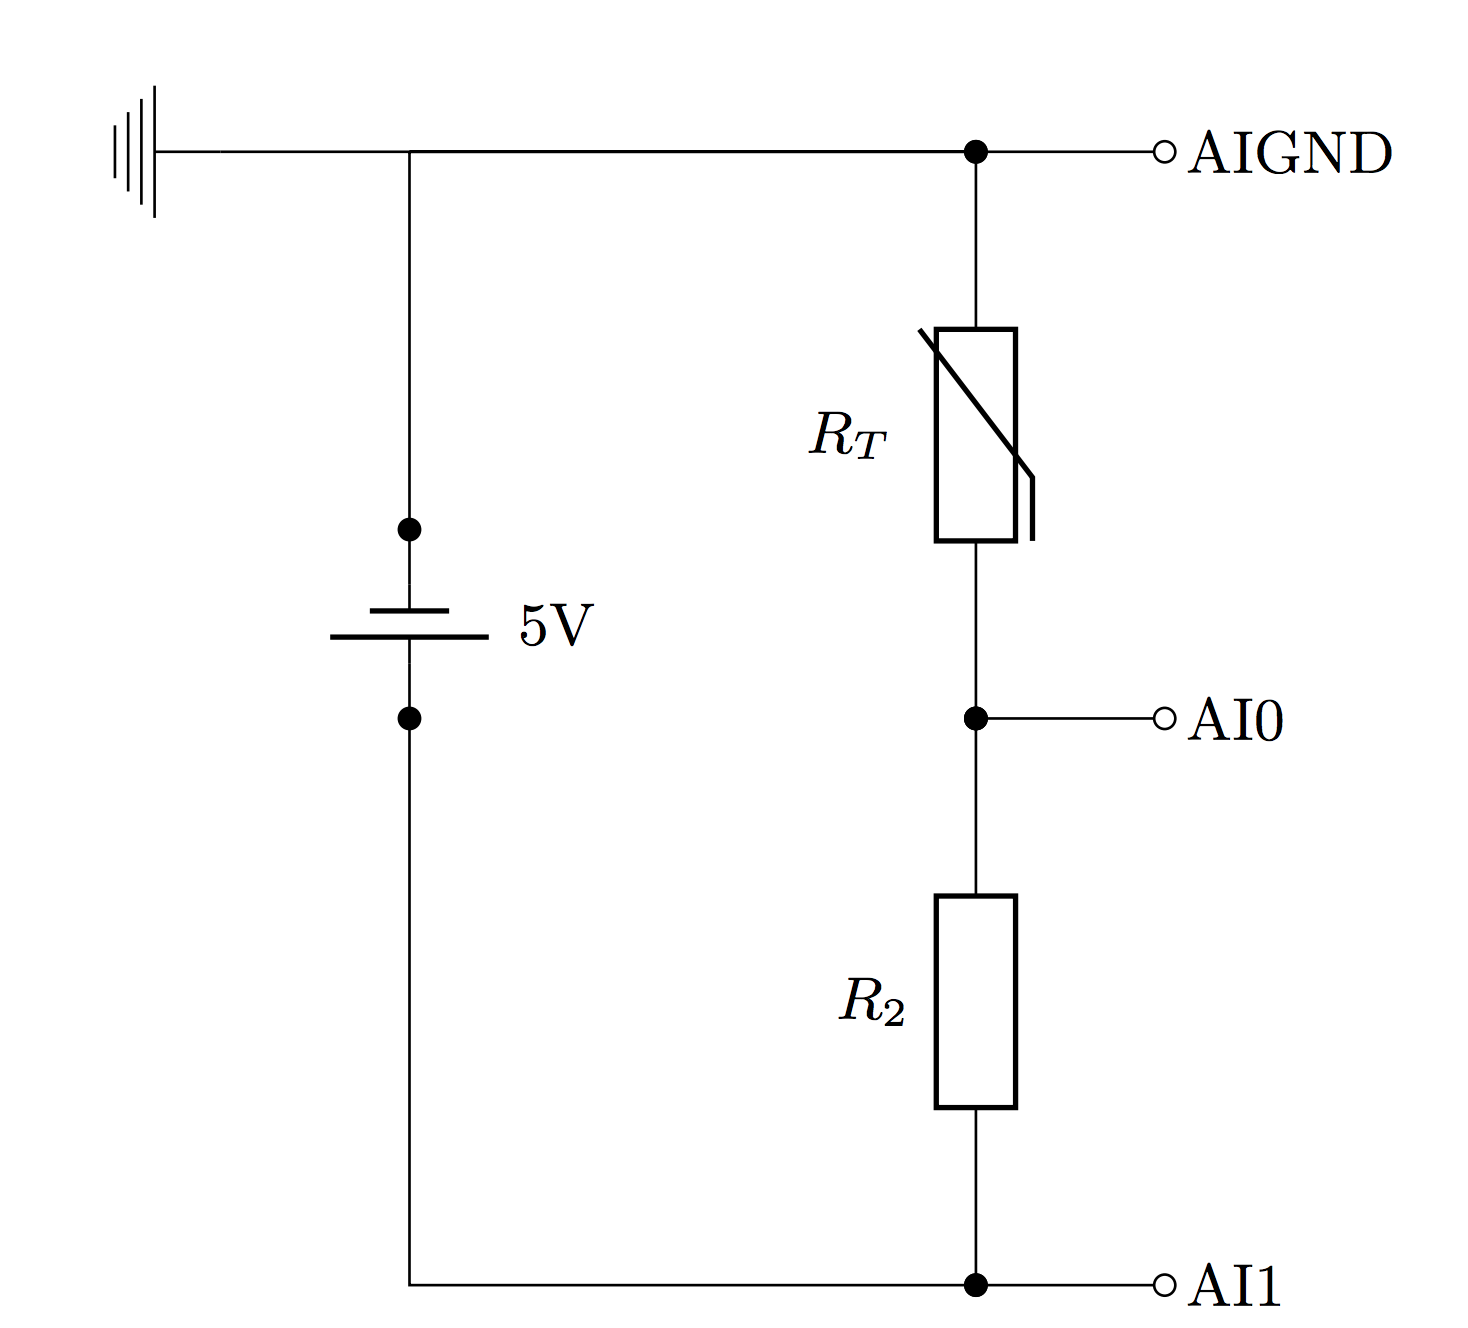
\includegraphics[scale=0.3]{fig_4.png}
    \caption{Krets brukt for å måle $R_T$ og sende informasjon fra kretsen til en datamaskin, som regner ut og plotter dataen \cite{oppgave}.}
    \label{fig4}
\end{figure}
Her er $R_T$ motstanden til en halvleder som er mer følsom mot temperaturforandring enn andre motstander. Ved at datamaskinen regner spenningsfallet over termistoren, og vet strømmen som går i kretsen, kan den regne ut resistansen til $R_T$ over tid, og dermed få data om temperaturen til termistoren. Først lot vi termistoren ikke oppleve temperaturforandring, for å se om resitansen var konstant, deretter varmet den opp ved kontakt med huden. \\
Hittil har vi brukt likestrøm (DC), men nå ønsker vi å gjøre eksperimenter med vekselstrøm (AC). Vekselstrømmen skal komme fra en funksjonsgenerator innebygd i oscilloscopet (PicoScope 2000 Series). Med funksjonsgeneratoren kunne vi variere amplitude og frekvensen til signalet fra datamaskinen. Vi koblet F$45$ inn i kretsen for å måle spenningen, her må multimeteret være stilt inn på AC. Vi sammenlignet så verdien vi leste av på F$45$, med verdien vi valgte for spenningen med oscilloscopet. Vi gjorde dette for signaler med sinus, sagtann og firkantsignal. \\
Til slutt ønsker vi å se på forholdet mellom to spenningsfallet i en RC krets med vekselstrøm som fungerer som et lavpassfilet på grunn av tregheten i kondensatoren, kretsen er vist i figur \vref{fig5}. Vekselstrømmen skal komme fra en funksjonsgenerator innebygd i oscilloscopet (PicoScope 2000 Series) og fra DA-omformer (digital-to-analog-omformer). Vi kunne henholdsvis lese av signalet på datamaskinen ved hjelp av en oscilloscopet og AD-omformer (analog-to-digital-omformer) for å gjøre målinger på kretsen.
\begin{figure}[h!]
  \centering
  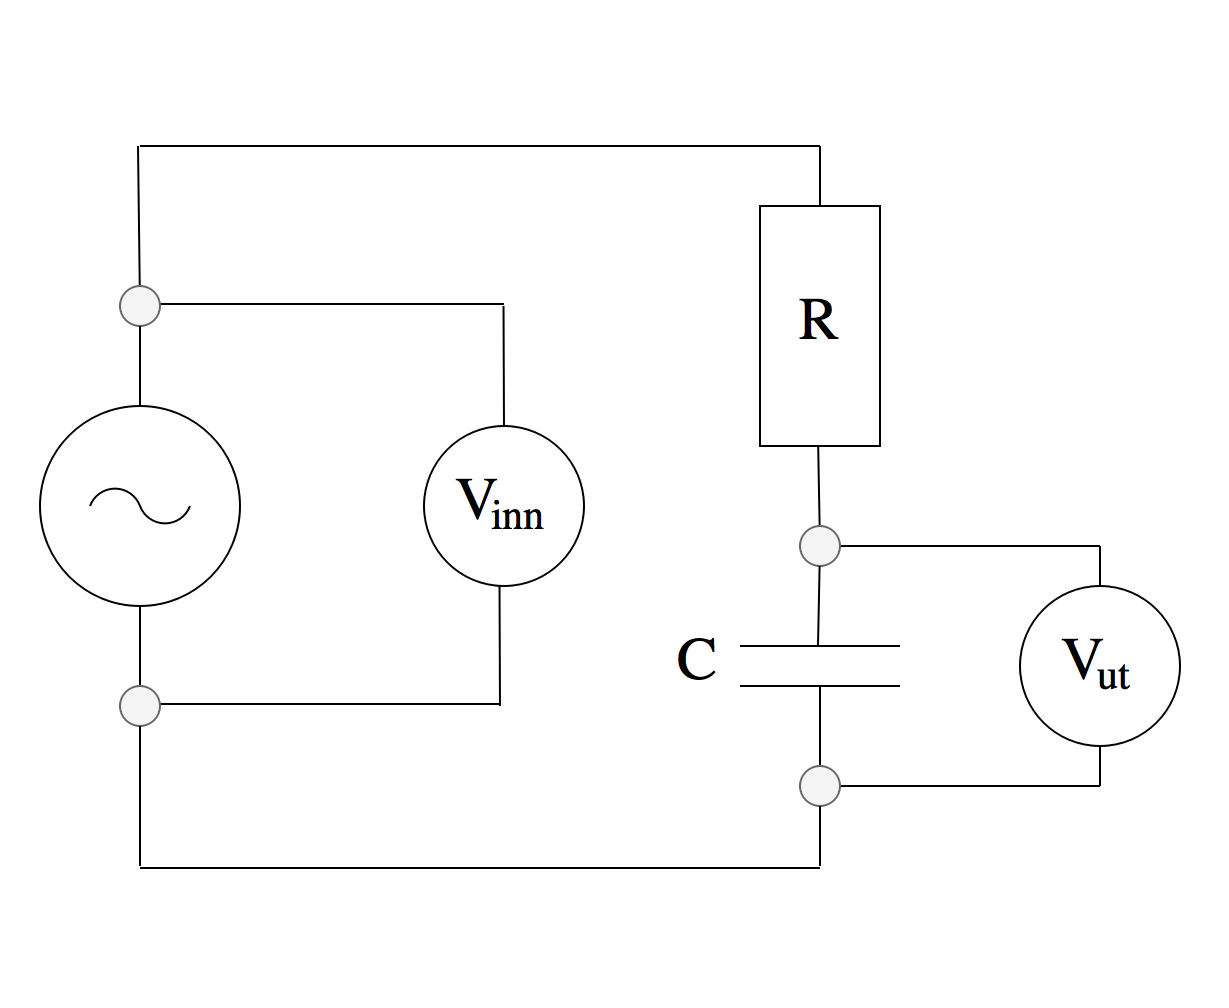
\includegraphics[scale=0.15]{fig_5.png}
  \caption{Krets brukt for å finne forholdet mellom $V_{inn}$ og $V_{ut}$ som blir forårsaket av tregheten i kondensatoren. De små sirklene ved batteriet representerer hvor vi koblet ledningene inn til først oscilloscopet, og senere til DA-omformeren for å generere signalet. De to små sirklene ved kondensatoren representerer hvor vi målte av dataen, først med oscilloscopet og senere med AD-omformeren for å sende data til datamaskinen.}
  \label{fig5}
\end{figure}
Som beskrevet i teoridelen (seksjon \vref{teori}) skaper kondensatoren en treghet i systemet hvis vi har en høy frekvens på spenningen i kretsen. For å gjøre målinger på denne effekten varierte vi frekvensen til et sinussignal fra spenningsgeneratoren logaritmisk fra $10$ til $10^6$ Hz, og gjorde noen ekstra målinger på området der vi merket forandring, som var for $500$, $5000$ og $50000$ Hz. Amplituden til signalet fra vekselstrømmen var på $\SI{706.5}{\milli \volt}$. For hver instilling noterte vi frekvens og amplitude til $V_{inn}$ og $V_{ut}$. Vi gjorde målingene først med oscilloscopet deretter med en AD-omformeren (anlog-to-digital-converter). Kapasitansen til kondensatoren var $\SI{100}{\nano\farad}$, og motstanden hadde resistans på $\SI{10}{\kilo\ohm}$.


\section{Resultater}
Resultater fra måling av kretsen vist i tabell \vref{table1}. Dataen i denne tabellen kommer fra avlesninger av kretsen vist i figur \vref{fig1}, der vi bare hadde måleapparatene F$45$ og F$75$ i krets med hverandre og varierte hva apparatene målte. Fra denne dataen kan vi se hvordan måleapparatet selv påvirker kretsen de selv er med i. \\
\begin{table}[h!]
\caption{Data fra elektrisk krets kunn med måleapparater  F$45$ og F$75$. Kretsen som dataen er hentet fra er vist i figur \vref{fig1}. Ut fra enhetene til verdiene målt finner du hva de målte av hverandre.}\centering
\label{table1}
{\renewcommand{\arraystretch}{1.2}
\begin{tabular}{|l|l|l|}
\hline
Fluke 75                 & Fluke 45                  & Rate F45 \\ \hline
$1.559 \pm 0.008$V       & $11.1 \pm 0.4 $M$\Omega$    & S        \\ \hline
$1.559 \pm 0.008$ V      & $11.100 \pm 0.031$M$\Omega$ & M        \\ \hline
$1.559 \pm 0.008$V       & $11.0 \pm 0.3 $M$\Omega$    & F        \\ \hline
$10.00 \pm 0.06$M$\Omega$  & $721.9 \pm 0.7 $mV       & S        \\ \hline
$10.00 \pm 0.06$M$\Omega$ & $0.7219 \pm 0.0004 $V   & M        \\ \hline
$10.02 \pm 0.06$M$\Omega$  & $0.720 \pm0.002$V         & F        \\ \hline
$0.000 \pm 0.001$V       & $0 \pm 1.5 \cdot 10^{-6}$ A     & S        \\ \hline
$0.000 \pm 0.001$V       & $0  \pm 3 \cdot 10^{-5}$ A      & M        \\ \hline
$0.000 \pm 0.001$V       & $0 \pm 3 \cdot 10^{-6}$ A       & F        \\ \hline
\end{tabular}
\end{table}
Kretsen vist i figur \vref{fig2} ble brukt til å måle resistansen til to motstander. Målingene vi gjorde er vist i tabell \vref{table2}. \\
\begin{table}[h!]
\centering
\caption{Data fra Fluke$45$ og Fluke$75$ som måler resistansen til to kjente motstander. Kretsen for målingene er vist i figur \vref{fig2}.}
\label{table2}
\begin{tabular}{c c c c}
\toprule
& $\Omega$ oppgitt & $\Omega$ målt    & $\Delta \Omega$    \\
\midrule
Fluke45 & $10\Omega$       & $10.141 \Omega$  & $\pm 33$ m$\Omega$ \\
Fluke75 & $10\Omega$       & $10.0\Omega$     & $\pm 0.2\Omega$    \\
Fluke45 & $1$ M $\Omega$   & $1.004$M$\Omega$ & $\pm 3.1$k$\Omega$ \\
Fluke75 & $1$ M $\Omega$   & $1.004$M$\Omega$ & $\pm 6$k$\Omega$   \\
\bottomrule
\end{tabular}
\end{table}
I kretsen vist i figur \vref{fig3} målte vi spenningen over batteriet og over resistansen, og vi målte strømmen ved et ampermeter. Ved hjelp av Ohm's lov \eqref{ohm} kunne vi regne ut resistansen til motstanden. Dataen fra denne måkingen er vist i tabell \vref{table3}.
\begin{table}[h!]
\centering
\caption{Målingene gjort på kretsen vist i figur \vref{fig3}}
\label{table3}
\begin{tabular}{c c c c }
\toprule
    Strøm $I$ (mA) & Spenning $V$ (V) & Resistans $R = V/I$ ($\Omega$) & Målested \\
\midrule
 0.0042 \pm 0.0015 &    4.22 \pm 0.03 &                  1.00 \pm 0.36 &      V_{inn} \\
 0.0046 \pm 0.0015 &    4.25 \pm 0.03 &                  0.92 \pm 0.31 &      V_R \\
 0.0060 \pm 0.0015 &    6.04 \pm 0.04 &                  1.01 \pm 0.26 &      V_{inn} \\
 0.0066 \pm 0.0015 &    6.04 \pm 0.04 &                  0.92 \pm 0.21 &      V_R \\
 0.0081 \pm 0.0015 &    8.22 \pm 0.05 &                  1.01 \pm 0.19 &      V_{inn} \\
 0.0089 \pm 0.0015 &    8.22 \pm 0.05 &                  0.92 \pm 0.16 &      V_R \\
\bottomrule
\end{tabular}
\end{table}
\subsection{Måle temperatur ved hjelp av resistanse}
Dataen fra kretsen vist i figur \vref{fig4} ble sendt til datamaskinen hvor vi kunne fremstlle temperaturen til termistoren som en funksjon av tid ved å regne ut resistansen med Ohm's lov \eqref{ohm}, og bruke \eqref{calc_temp} til å finne temperaturen. Grafen vist i figur \vref{fig6} viser hvordan temperaturen endrer seg over tid.
\begin{figure}[h!]
  \centering
  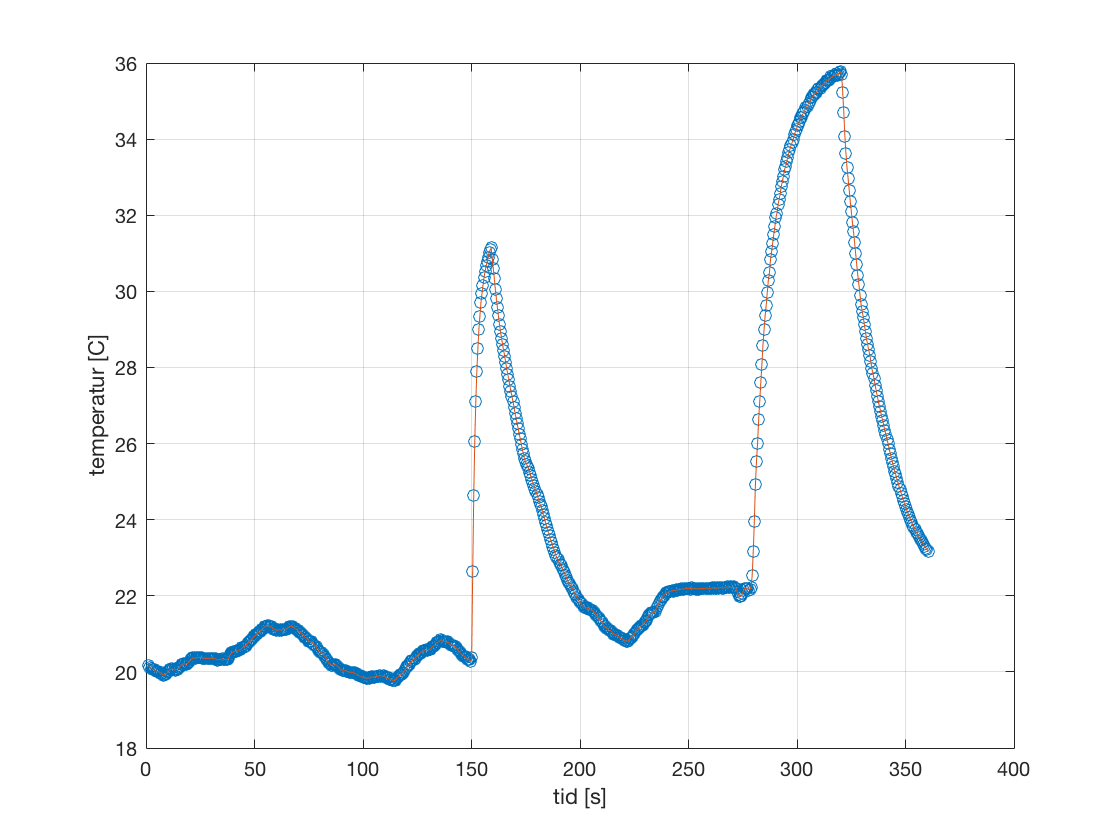
\includegraphics[scale=0.15]{fig_6.png}
  \caption{Temperaturen til termistoren som en funksjon av tid. Hver sirkel representerer en måling. Vi kan med dette lettere se hvor rask endringen er. Den oransje linja under er en linje trukekt mellom hver måling.}
  \label{fig5}
\end{figure}

\subsection{Vekselspenning med frekvensgenerator, oscilloscop og multimeter}
I den elektriske kretsen vist i figur \vref{fig5} varierte vi formen på signalet mellom sinus, sagtann og firkant-signal. Da vi leste av målingene gjort med oscilloscopet fant vi dataen vist i tabell \vref{}.

\begin{table}[h!]
\centering
\caption{Målingene gjort på kretsen vist i figur \vref{fig5}. Her er Amplituden den vi valgte på oscilloscopet, F$45$ er verdien vi leste av multimeteret, og RMS er RMS veriden til signalet, utregnet av oscilloscopet.}
\label{table5}
\begin{tabular}{c c c c}
\toprule
    Signalform & Amplitude $V$ (V) & F$45$ $V$ (mV)  & RMS \\ \hline
\midrule
 Sinus   &    1  &                  705.79 \pm 2.41 &      705.7 \pm 2.5 \cdot 10^{-4} \\
 Firkant &    50 &                  49.627 \pm 0.20 &      50.6 \pm 0.0024\\
 Sagtann &    2  &                  1.1419 \pm 0.0214 &    1.149 \pm 3.5 \cdot 10^{-4}  V_{inn} \\ \hline
\bottomrule
\end{tabular}
\end{table}

\section{Diskusjon}
\subsection{Måling av multimetere}
Fra dataen vist i tabell \vref{table1} ser vi at det er null i de tre nederste radene. Fra dette kan vi trekke slutningen at det ikke kreves å sende strøm gjennom en krets for å måle spenning og strøm, i motsetning til måle-kombinasjonen ovenfor i tabellen. Vi ser også at voltmeteret i F$75$ har en resistanse på $11.1M\Omega$. For at det ikke skal gå noe strøm gjennom voltmeteret er det viktig at voltmeteret har en stor resistanse, og det gjelder for F$75$. Hvis resistansen F$75$ måler spenningsfallet over begynner å nærme seg $11.1M\Omega$ vil det være en merkbar effekt i kretsen på grunn av påvirkningen til voltmeteret fra F$75$. Andre veien ser vi at reistansen til F$45$ er på $10M\Omega$, og akkurat de samme poengene gjelder her. Vi ser også fra dataen at måleapparatene sender en strøm inn i kretsen for å klare å måle av resistanse, men ikke for å måle av spenning eller strøm. \\
\subsection{Motstand, likestrøm og likespenningsmålinger med multimeter}
Når vi ser på dataen vist i tabell \vref{table3} over måling av resistansen til motstanden på $1$M$\Omega$ ser vi at det er mye mer nøyaktig å regne ut resistansen til motstanden ved hjelp av spenningen målt på $V_{inn}$ enn ved spenning målt over $V_r$. Grunnen til dette er at her er resistansen $R$ til motstanden var av samme størellsesorden med motstanden i voltmeteret, som vi fant tidligere at var på $11.1$M$\Omega$. For at et voltmeter skal gjøre jobben sin godt må motstanden over voltmeteret være mye større enn motstanden over kompenten den måler over. Siden den ikke er det i dette tilfellet vil det gå mindre strøm gjennom resistansen, og vi får målt en lavere resistanse på motstanden. Siden vi ikke hadde nok måleapparater målte vi ikke spenningsfallet over batteriet og spenningsfallet over resistansen samtidig. Derfor var, når vi målte spenningsfallet over kretsen, tilnærmet lik bare fra motstanden på $1$M$\Omega$, siden motstanden fra amperemeteret er neglisjerbar. Vi ser fra tabellen \vref{table3} at vi får mye mer nøyaktig måling av å regne ut motstanden ved å bare se på målinger fra $V_{inn}$.
\subsection{Automatiserte målinger av termistor-motstand}
Av å måle termistormotstanden klarte vi å finne temperaturen til termistoren over tid.
\subsection{Vekselspenning med frekvensgenerator, oscilloscop og multimeter}
Fra dataen vist i tabell \vref{table5} ser vi at verdien vi måler fra multimeteret er lik RMS verdien til signalet. RMS-veriden represneterer 



\begin{thebibliography}{9}
\bibitem{squires}
Squires, G.L. \emph{Practical Physics}, Cambridge University Press, 2001.
\bibitem{skaar}
Skaar, J. \emph{Elektromagnetisme}, 2017
\bibitem{oppgave}
Dysthe, D.K\,\, Røyne, A.\,\, Ulven, O.I \emph{Strøm og spenning}, 2018

\bibitem{rms_wiki}
Wikipedia \emph{Root mean square}, 07.02.2018

\end{thebibliography}
\end{document}
%
% ****** End of file apssamp.tex ******
